\section{Location, Type, Age, Space Programming, Energy Code, and Change Over Time}[!ht]
\subsection{Location}

ComStock has four levels of location granularity for its building models: ASHRAE Standard 169 - 2006 climate zone, census division, state, and county. During sampling, each model is first assigned a climate zone, then a county, then a state and census division. The climate zone and county probability distributions come from the CoStar and HIFLD data provided by the Homeland Security Infrastructure Program (HSIP) on a building count basis. The state and census division are assigned using a lookup table that is based on the model's sampled county. The location metadata impacts numerous characteristics in the model, such as weather file, building type, building geometry characteristics (e.g., number of stories and rentable area), and energy code applicability. Table  \ref{tab:census_division_models_table} shows the number of models used in each census division.

Additional location metadata is joined to the \emph{buildstock.csv} for use in parsing ComStock results. This includes data such as \href{https://www.census.gov/programs-surveys/geography/guidance/geo-areas/pumas.html}{Public Use Microdata Area} (PUMA), \href{https://www.energy.gov/eere/buildings/building-america-climate-specific-guidance}{Building America climate zone}, \href{https://isorto.org/}{independent system operator (ISO) region}, and \href{https://www.nrel.gov/analysis/reeds}{ReEDS balancing area}. This location metadata is joined on the \href{https://www2.census.gov/geo/pdfs/education/CensusTracts.pdf}{census tract} level. Census tracts are assigned to the \emph{buildstock.csv} using the CoStar and HSIP data.

\begin{table}[h!]
\centering
\small
\caption[Distribution of ComStock Models in Each Census Division]{Distribution of ComStock Models in Each Census Division}
\label{tab:census_division_models_table}
\begin{tabular}{|c|c|c|}
\hline
\textbf{Census Division}                                & \textbf{Count}              & \textbf{Percentage}                                     \\ \hline
East North Central                                         & 54122                 & 15.46\%      \\ \hline
East South Central                                         & 19882                 & 5.68\%      \\ \hline
Mid-Atlantic                                         & 44976                & 12.85\%      \\ \hline
Mountain                                         & 24258                & 6.93\%      \\ \hline
New England                                         & 16791                & 4.80\%      \\ \hline
Pacific                                         & 54799                & 15.66\%      \\ \hline
South Atlantic                                         & 72616                & 20.75\%      \\ \hline
West North Central                                         & 20910                & 5.97\%      \\ \hline
West South Central                                         & 41646                & 11.90\%      \\ 
\hline
\end{tabular}
\end{table}

\subsection{Building Type}
\label{sec:building_type_meta}

The building types used by ComStock were originally defined by the DOE reference buildings, which were extended to create the prototype buildings. These building type definitions represent buildings by drawing on the applicable building code sets. Both the reference buildings and the prototype buildings have historically been used by building code organizations, include the ASHRAE 90.1 committee, to understand the potential impact of various code updates on newly constructed buildings.

Each building type is predominantly defined by a space type breakdown. For a given square footage of a ComStock building type, the fraction of the square footage of space type A (open office) vs. B (closed office) will remain the same as what they are in the DOE prototype models with two exceptions. Although these definitions are useful in the analysis of energy codes, there are several cases where they fail to provide the variability required for ComStock to provide a useful representation of the U.S. commercial building stock. There are two building types are currently represented with additional variability in space programming - large office and strip malls.

\begin{description}
\item[Large Offices] Currently, large offices have variable data-center loads in ComStock. This aligns with study data obtained through the \href{https://www.nrel.gov/docs/fy22osti/80889.pdf}{End-Use Load Profiles} (EULP) project that was used to calibrate ComStock. This results in a higher degree of EUI variability within the large office building type than would be expected with only a change in space programming, given the high energy intensity of the data center space type.
\item[Strip Malls] Strip malls often contain one or more restaurants. Strip malls with restaurants often have significantly higher EUIs than restaurant-free strip malls, which are the only kind represented by the reference and prototype models. To address the significant lack of diversity and variability in strip mall EUIs, the End-Use Load Profiles project added a variable restaurant component to strip mall models in ComStock. This results in a more realistic distribution of loads by end use across the strip mall segment.
\end{description}

\subsection{Vintage}

Vintage, as previously discussed in the sampling section~\ref{Characteristic Estimation}, is a key component of ascertaining the age and associated efficiency of building components. Vintage is determined based on information from either CoStar or HIFLD. However, in many cases, the vintage must be inferred due to a lack of available data on a county or state basis. When there is insufficient data on a county basis, state data are used, and in the few cases (typically in relation to hospitals) where state data are unavailable, national data are used.

Commercial buildings are complex in that each subsystem of the building---except perhaps walls---is expected to be replaced or updated at least once during the life of the building, without the building being reconstructed from the ground up. As such, it is critical to understand the year in which a building was first constructed in order to estimate the age (and the associated minimum energy code) as a function of the vintage. The latest year of intervention is calculated for each building component as a function of the vintage, and each of these are passed to an energy code lookup to determine which, if any, energy codes were in force.

Finally, it is important to note that vintage is especially important for recent construction. Buildings built within the last decade are unlikely to have significantly different or updated systems compared to those used at the time of construction. As a result, these buildings are a unique stock segment and have potential for cost-effective impact in the commercial building stock.

\subsection{Energy Code} % Andrew
\label{sec:energy_code}

\paragraph{Energy Code Adoption}
Some states have a statewide code, while others have codes that are determined at the city or county level. For ComStock, the adoption of an energy code is assumed to be a function of year and state. For states with no statewide code, ComStock selects the code covering the biggest cities in the state. Where a state code was not a derivative of the ASHRAE 90.1 series of codes, the most similar versions of ASHRAE 90.1 were used for that state. The exception to this is California, where the Title 24 series of codes, as represented in DEER \citep{cpuc_deer}, was used because this series of codes was known to be significantly different from ASHRAE 90.1. Most of the information used to develop the code adoption history was taken from the Building Codes Assistance Project \citep{building_codes_assistance}. Much of the building stock was constructed before energy codes were widespread. For this time period, the ``energy code'' is described as either ``DOE Ref Pre-1980,'' whose assumptions are drawn from \cite{doe_reference_buildings}, or ``DOE Ref 1980-2004,'' whose assumptions are a combination of ASHRAE 90.1-1989 and \cite{doe_reference_buildings}. Details on the specific assumptions for each energy code are described in more detail throughout this document. The code adoption history assumptions are shown in Figure~\ref{fig:energy_code}.

\begin{figure}
  \centering
  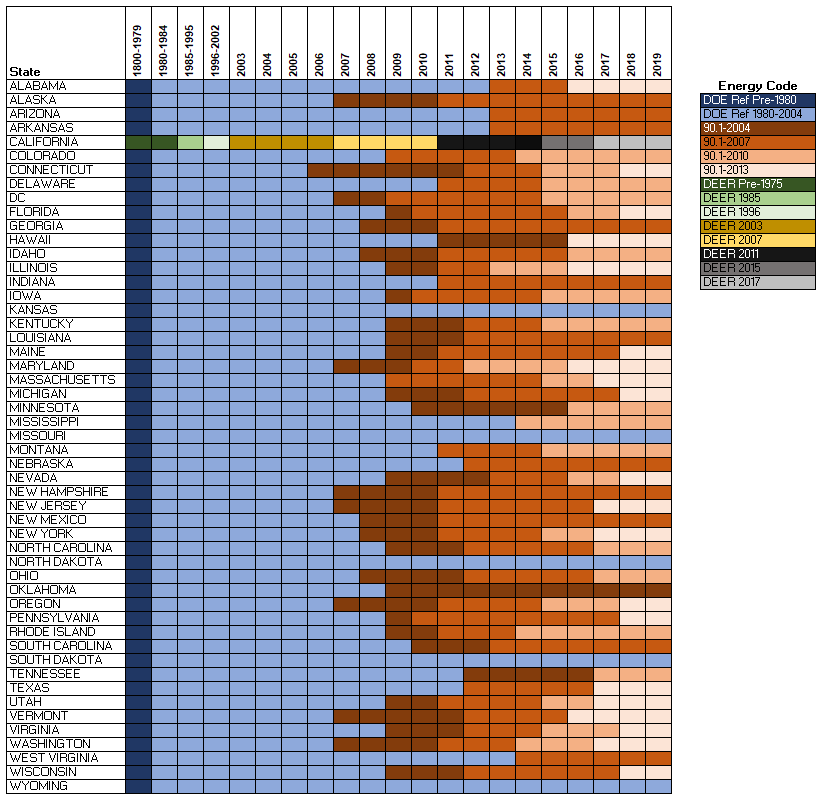
\includegraphics[]{figures/energy_code.png}
  \caption{Adoption of energy codes by state over time.}
  \label{fig:energy_code}
\end{figure}

\paragraph{Energy Code Compliance}
For this discussion, energy code compliance is defined as the extent to which a building constructed to comply with a certain energy code meets the requirements of that code. For example, a building built to comply with ASHRAE 90.1-2010 may meet all envelope requirements but fail to meet some HVAC control requirements. Unfortunately, there is little information available on commercial energy code compliance at a national level, and the information that does exist is not detailed. The status of this information is described in a detailed report \citep{icf_com_code_compliance_status} generated for EIA’s NEMS modeling effort. What we do know, both from this information and anecdotally, is that commercial energy compliance is imperfect. Some buildings and building systems exceed code, and others lag behind. Because of the data limitations, we assume that all building systems meet the requirements of the energy code that was in force in their location when the building was originally constructed and as the building systems were replaced over time. As data on major building systems become available we hope to move away from this code-compliance-based framework toward a model driven by distributions of known building characteristics.

\subsection{Building System Turnover and Effective Useful Life} % Andrew
\label{sec:system_turnover_and_eul}

We assume that all major building systems are installed when the building is constructed, and that they are replaced periodically over the lifespan of the building. Replacements may be made because of equipment failure, building remodeling, energy efficiency upgrades, etc. To model the turnover of building systems, it is necessary to understand how often these building systems are replaced, which determines how long they last in the building stock. The metric commonly used by the energy efficiency community to describe the lifespan of a measure is effective useful life (EUL). The California Public Utilities Commission defines EUL as ``an estimate of the median number of years that the measures installed under the program are still in place and operable'' \citep{cpuc_ee_manual}. In the reliability community, EUL is typically referred to as ``median time to failure'' \citep{ti_reliability_website}, whereas ASHRAE uses the term ``median service life'' \citep{ashrae_reliability_db_article}.

\par
For ComStock, the primary source of EULs is the California Public Utilities Commission (CPUC) Database of Energy Efficiency Resources (DEER) \citep{cpuc_deer}. Previous work on EULs indicates that there is wide variation in the quality of national EUL data, but it also indicates that the studies performed in DEER are generally the best available \citep{what_makes_good_eul}. The values in DEER were cross-referenced against the lifetimes used in the EIA NEMS Commercial Demand Module \citep{nems_com_demand_module} and the ASHRAE Service Life and Maintenance Cost Database \citep{ashrae_reliability_db}. Table~\ref{tab:effective_useful_life} shows the EULs assumed for different building systems in ComStock.

\begin{table}
\small
\caption[Effective Useful Life of Major Commercial Building Systems]{Effective Useful Life of Major Commercial Building Systems}
\label{tab:effective_useful_life}
\centering
\begin{tabular}{|p{3cm}|p{1cm}|p{11cm}|}
\hline
\textbf{Major Building System}                       & \textbf{EUL (Years}) & \textbf{Notes} \\
\hline
Envelope---Wall Insulation                  & 200         & This value was based on engineering judgment. DEER EULs are capped at 20 years, per CPUC policy. NEMS does not appear to model wall turnover separate from whole-building replacement.\\
\hline
Envelope---Roof Insulation                  & 200         & This value was based on engineering judgment. DEER EULs are capped at 20 years, per CPUC policy. NEMS does not appear to model roof turnover separate from whole-building replacement.\\
\hline
Envelope---Windows                          & 70          & Based on a reliability analysis of windows from the 2014 Commercial Building Stock Assessment from the Pacific Northwest. DEER uses an EUL of 20 years for window replacement, as the DEER EULs are capped at 20 years, per CPUC policy.\\
\hline
Exterior Lighting                           & 15          & This closely matches the highest EUL in DEER for outdoor lighting (16 years). NEMS does not break out exterior lighting, but all NEMS commercial lighting technology types have a 10-year EUL.\\
\hline
Interior Lighting                           & 10          & This is in line with the EULs in DEER for interior lighting, and matches the 10-year EUL for all commercial lighting technologies in NEMS.\\
\hline
HVAC                                        & 20          & The highest EUL in DEER for HVAC is 20 years. For rooftop air conditioners, which serve by far the largest portion of the building stock, NEMS uses a 21-year EUL. NEMS HVAC EULs range from 9.5 years for window AC units up to 30 years for some boilers. \citet{ashrae_reliability_db} includes 33 packaged DX rooftop units with a mean lifetime of 21 years, and appears to be the source of some NEMS HVAC lifetimes.\\
\hline
Service Water Heating (SWH)                 & 15          & The highest SWH EUL in DEER is 20 years for a tankless water heater. Most tank-based SWH equipment in DEER has an EUL of 15 years or less. NEMS non-solar SWH equipment EULs range from 10 to 15 years. \citet{ashrae_reliability_db} includes 5 gas-fired water heaters with a mean lifetime of 15 years, and 36 electric water heaters with a mean lifetime of 10 years.\\
\hline
Interior Equipment (Plug and Process Loads) & 15          & This value was based on engineering judgment and is meant to represent an average over all types of plug and process loads. If plug and process loads are addressed in future iterations, splitting the plug and process loads into information technology (IT) equipment and other equipment will be investigated, as IT equipment typically has a higher turnover rate than other process loads, such as hospital equipment or commercial kitchen equipment. NEMS includes commercial kitchen equipment with an EUL of 12 years, commercial ice machines with an EUL of 8 years, commercial vending machines with an EUL of 13.5 years, and commercial refrigeration equipment with an EUL of 10 years. \\
\hline
\end{tabular}
\end{table}

\subsubsection{Building Envelope}
For the building envelope (windows, wall insulation, and roof insulation), the DEER database was not informative, because the maximum EUL is capped at 20 years, per CPUC policy. Because of this, we sought out other sources of envelope lifetime information.

\paragraph{Windows}
As part of the DOE-funded Advanced Building Construction initiative, a team collected information on windows from a variety of commercial building surveys, including a new survey of buildings built since roughly 2010. Unfortunately, while most of the surveys did ask about windows, only one survey had enough information to perform a reliability analysis (because windows are long-lived). This survey was the 2014 Commercial Building Stock Analysis \citep{neea2014cbsa}, which covers the Pacific Northwest. This survey included information on the age of the building, whether the windows had ever been replaced (and if so, an estimate of the year of replacement), and a weighting factor to describe how each sample fit into the whole building population. From these data, we performed a reliability analysis. Figure~\ref{fig:comWindowSurvivalCurve} shows the estimated survival curve. As indicated by the black cross mark on the figure, the EUL estimate for windows is 70 years. However, the maximum lifespan extends to more than 400 years. In practice, this indicates that windows on some buildings will never be replaced.

\begin{figure}
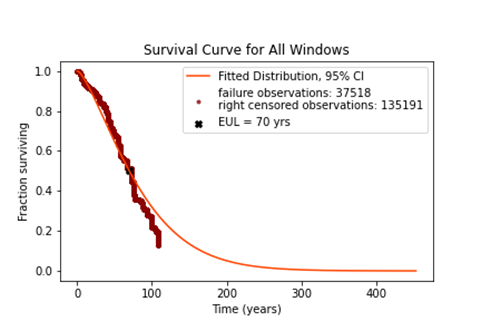
\includegraphics[width=0.6\textwidth]{figures/window_survival_curve.png}
\centering
\caption[Reliability analysis for windows in commercial buildings]{Reliability analysis for windows in commercial buildings, from 2014 CBSA \citep{neea2014cbsa}.}
\label{fig:comWindowSurvivalCurve}
\end{figure}

\paragraph{Walls and Roofs}
None of the data sources we identified included information on EULs for walls and roofs, or, more specifically, the insulation on these surfaces. DEER EULs are capped at 20 years, per CPUC policy. NEMS does not appear to model wall turnover separately from whole-building replacement. Based on engineering judgment, we selected an EUL of 200 years to indicate that for most buildings, the wall and roof insulation will not be replaced before the building is demolished.

\subsubsection{Distribution of Lifespans}
The EUL estimates in Figure \ref{fig:comWindowSurvivalCurve} represent the median lifespan for a given building system. However, not all systems will fail and be replaced after exactly that amount of time. To represent this diversity of failure rates we use a distribution.

\par
The simplest approach would be to use a normal distribution centered on the EUL. However, studies of reliability data show that this is not a good assumption; instead, these studies often use a Weibull distribution to represent lifetimes. To check whether a Weibull distribution accurately represented the lifetimes of building equipment, we performed a reliability analysis on data from the ASHRAE Service Life and Maintenance Cost Database \citep{ashrae_reliability_db}. This analysis was performed following the methodology described in an ASHRAE journal article \citep{determine_equip_life}, and was implemented using the reliability package \citep{matthew_reid_2020_3938000} in Python. Four categories of equipment with a reasonable number of entries were investigated: air handling units, boilers, chillers, and air source DX equipment (all types of each available in the database).

\begin{figure} [ht!]
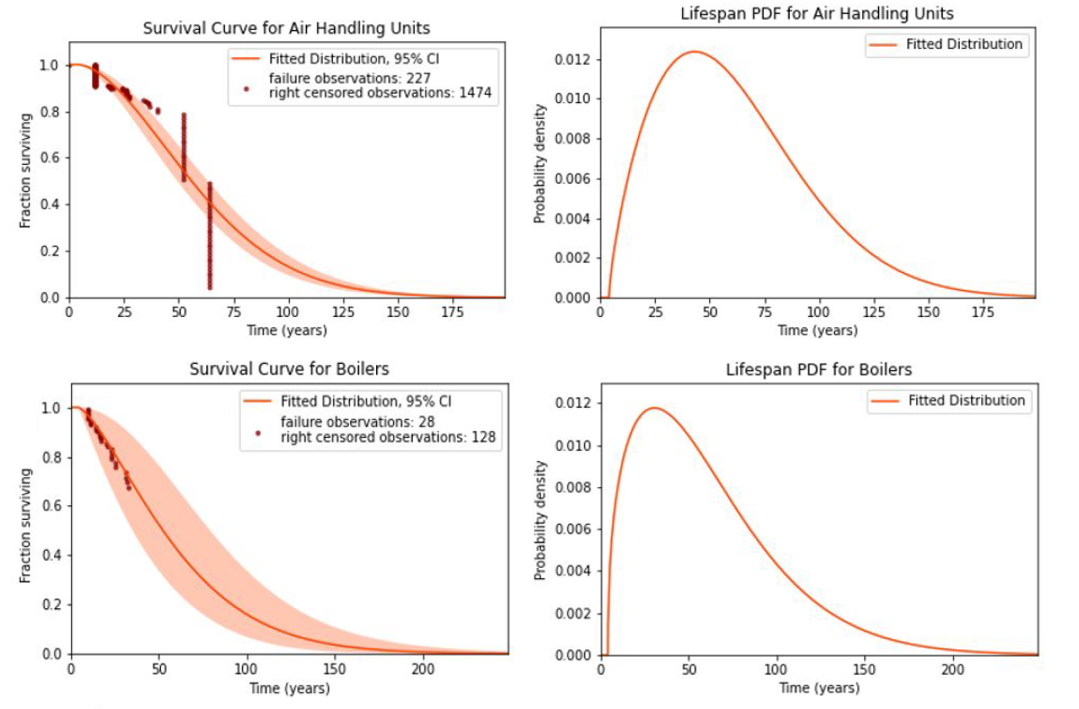
\includegraphics[width=\textwidth]{figures/ashrae_equip_lifespans2.png}
\centering
\caption[Survival curves and derived lifespan probability density functions for HVAC equipment]{Survival curves and derived lifespan probability density functions for commercial HVAC equipment.}
\label{fig:hvac_survival_curves}
\end{figure}

As shown in Figure~\ref{fig:hvac_survival_curves}, Weibull distributions are a good fit for several categories of HVAC equipment failure data. Although the ASHRAE database includes data for many different types of HVAC equipment, it was not selected as the primary source for deriving EULs for ComStock due to the limitations and biases in the database described by its creators \citep{ashrae_reliability_db_article}.
Instead, we decided to use the EUL sources described in Table~\ref{tab:effective_useful_life} and develop Weibull curve parameters around these EULs. The selected parameters are shown in Table~\ref{tab:eul_distributions}. For the 70-year EUL, the parameters came from the window reliability analysis. For the 10-, 15-, and 20-year EULs, the only constraint was to match the EUL definition: 50\% of the equipment would still be operable at the EUL. A minimum lifespan of 60\% of the EUL was selected with the assumption that although individual components of a system might fail, it is unlikely that products on the market routinely fail at a whole-building scale in only a few years. The 200-year EUL parameters were selected to represent no failure for the life of the building.

\begin{table}
\small
\centering
\caption[Commercial Equipment Lifetime Weibull Distribution Parameters]{Commercial Equipment Lifetime Weibull Distribution Parameters}
\label{tab:eul_distributions}
\begin{tabular}{|c|c|l|l|}
\hline
\textbf{EUL} & \textbf{Shape (beta)} & \textbf{Scale (alpha)} & \textbf{Shift (gamma)}    \\ \hline
10  & 1.6          & EUL / 2 = 5     & EUL * 0.6 = 6  \\ \hline
15  & 1.6          & EUL / 2 = 7.5   & EUL * 0.6 = 9  \\ \hline
20  & 1.6          & EUL / 2 = 10    & EUL * 0.6 = 12 \\ \hline
70  & 1.3          & 91              & 0              \\ \hline
200 & 1.0          & 1               & 200            \\ \hline
\end{tabular}
\end{table}

\subsection{Space Type Ratios}
\label{sec:space_type_ratios}
A space type refers to a portion of a building that has a distinct usage, purpose, occupancy schedule, thermostat set point, etc. Most buildings have multiple space types. For example, schools typically have classrooms, hallways, restrooms, cafeterias, etc. In ComStock, each building type is assumed to have a fixed ratio of various space types relative to the total building floor area. For buildings outside of California, the space type ratios were largely taken from the DOE commercial reference building models \citep{deru_2011}. For buildings in California, the space type ratios were largely taken from the DEER prototype models \citep{cpuc_deer}. There are certain building types that have altered ratios or are a mix of building types. For example in ComStock, warehouses include both unconditioned storage facilities and light manufacturing. Warehouse building subtypes alter the ratio of bulk storage. Retail strip mall buildings have different ratios of restaurant space types, with the default being 20\%. Two examples of space type ratios are shown in Table \ref{tab:space_type_ratios}. See Table~\ref{tab:space_type_ratios_all} for the space type ratios for all building types.

\begin{table}
\small
\caption[Space Type Ratio Example]{Space Type Ratio Example}
\label{tab:space_type_ratios}
\centering
\begin{tabular}{|l|l|l|c|}
\hline
\textbf{Building Type} & \textbf{Building Subtype} & \textbf{Space Type} & \textbf{Ratio} \\ \hline
Warehouse & warehouse\_default & Bulk & 66\% \\ \hline
Warehouse & warehouse\_default & Fine & 29\% \\ \hline
Warehouse & warehouse\_default & Office & 5\% \\ \hline
Retail Strip Mall & strip\_mall\_restaurant20 & Strip mall - type 1 & 20\% \\ \hline
Retail Strip Mall & strip\_mall\_restaurant20 & Strip mall - type 2 & 20\% \\ \hline
Retail Strip Mall & strip\_mall\_restaurant20 & Strip mall - type 3 & 40\% \\ \hline
Retail Strip Mall & strip\_mall\_restaurant20 & Dining & 15\% \\ \hline
Retail Strip Mall & strip\_mall\_restaurant20 & Kitchen & 5\% \\ \hline
\end{tabular}
\end{table}

\subsection{Weather Data}
ComStock can be run with two different types of weather data: typical meteorological year (TMY3) and actual meteorological year (AMY). AMY data is the data measured during a specific year, taken from weather stations such as those at airports. Because these data are from a particular calendar year, weather patterns that span large areas, such as nationwide heat waves, are captured in the data across multiple locations. Therefore, these weather patterns are captured in the outputs of ComStock. This is important for use cases where coordinated weather patterns influence loads, such as peak load impacts for bulk power grid planning. TMY3 data, in contrast, take the ``most typical'' weather for each calendar month from a 30-year historical record and stitch these months together to form a complete year. The advantage of this method is that the weather data is less influenced by an extremely hot or cold year. However, this approach does not capture wide-area weather patterns, as the month of data used varies from location to location. For a more in-depth discussion of AMY and TMY3 weather data, see \cite{eulp_final_report}.

For geographic granularity, ComStock currently uses one weather file for each county in the United States. For counties with no weather data available (generally sparsely populated rural areas), data from the nearest weather station in the same climate zone are used. See \citep{eulp_final_report} for a more in-depth discussion of the weather data sources, cleaning process, and assignment assumptions.